\chapter{Evaluation}

As mentioned in Chapter 4 there is no reliable baseline and one needs to be established first with some basic CNN architectures. Then different architectures will be compared against each other with and without pre-training in order to find out if transfer learning is a valid option for this problem task. Data augmentation should add regularization and lead to a model that is better generalizable to the test set. New architectures will then be created to fit better the problem at hand. \\

The learning rate decay is defined as reducing the learning rate by a factor of 10 every N epochs and holds true for all the experiments: \\

\[ lr = lr * (0.1^{\frac{epoch}{decay}}) \] \\

For the baseline, I used a grid search approach in optimizing the learning rate and the learning rate decay. For all later architectures, I used Sigopt which utilizes bayesian optimization. With SIgopt I followed the official guideline to run the model for 10 times for every hyperparameter which needs to be optimized. For Alexnet and all state-of-the-art architectures I optimize the following three hyperparameters: learning rate [0.0001 - 0.1]; momentum [0 - 1]; weight\_decay [0.00001 - 0.01]. \\

Preliminary runs have shown that 50 epochs are long enough to converge as will be shown for every architecture separately. \\

The remaining of this chapter is in the following format. I introduce the optimized hyperparameters for each architecture and show the achieved accuracies. I compare the results with transfer learning and discuss the graphs and confusion matrices. For transfer learning a separate optimization with Sigopt is performed, since the hyperparameters need to be different if the starting point of the model is not randomly defined. Then I will attempt to shed some light into what exactly was learned by showing some of the visualizations.

\section{CNN\_Basic - Baseline}

For the baseline, a simple 3-layered CNN was chosen with three convolutions and no maxpooling. For the activation function, a leaky ReLU is applied after each convolution. A simple grid search is applied to the model as seen in table \ref{tbl:cnn-basic-baseline}. The best result is achieved with a rather small learning rate of 0.0005 and an lr-decay of 20.

\begin{table*}[h]
    \ra{1.3}
    \caption{Accuracy (\%) for several learning rates and lr-decays for CNN\_Basic as a baseline.}
    \centering
    \begin{small}
    \textsc{
      \resizebox{0.99\textwidth}{!}{%
      \begin{tabular}{rcclcclcc}
      \toprule 
      & \multicolumn{2}{c}{Learning-Rate decay: 10} && %
        \multicolumn{2}{c}{Learning-Rate decay: 15} && %
        \multicolumn{2}{c}{Learning-Rate decay: 20} \\
      \cmidrule{2-3} \cmidrule{5-6}  \cmidrule{8-9}
      & learning rate & accuracy  && %
        learning rate & accuracy  && %
        learning rate & accuracy  \\ 
      \midrule
      CNN\_BASIC        & 0.1 & 69.10\%  &&  0.1 & 65.78\% &&  0.1 & 64.78\% \\
      CNN\_BASIC        & 0.05 & 63.46\%  &&  0.05 & 67.44\% && 0.05 & 65.78\% \\
      CNN\_BASIC        & 0.01 & 69.77\%  &&  0.01 & 70.10\% &&  0.01 & 69.77\% \\
      CNN\_BASIC        & 0.005 & 68.44\%  &&  0.005 & 71.43\% &&  0.005 & 72.09\% \\
      CNN\_BASIC        & 0.001 & 72.43\%  &&  0.001 & 70.10\% &&  0.001 & 74.42\% \\
      CNN\_BASIC        & 0.0005 & 73.75\%  &&  0.0005 & 73.42\% &&  \textbf{0.0005} & \textbf{76.74\%} \\
      CNN\_BASIC        & 0.0001 & 68.11\%  &&  0.0001 & 70.76\% &&  0.0001 & 70.43\% \\
    \bottomrule
    \end{tabular}}
    }
    \end{small}
    %\end{center}
    \vspace{-3.9mm}
    \label{tbl:cnn-basic-baseline}
\end{table*}

\quad


These results are much better than expected and should not be that high since the image size is resized to 32 by 32 pixels. As seen in figure \ref{fig:cnn-basic} the training accuracy achieves 94.54\% while the validation accuracy achieves 71.42\%. Such a big difference between training accuracy and the final test accuracy of 76.74\% means that the model overfitted strongly to the training data, learning it too well and thus decreasing generalizability. Having the accuracies for validation and test sets near each other is good and means that the validation set is representable of the test set.

\begin{figure}[h]
\centering
\subfigure{
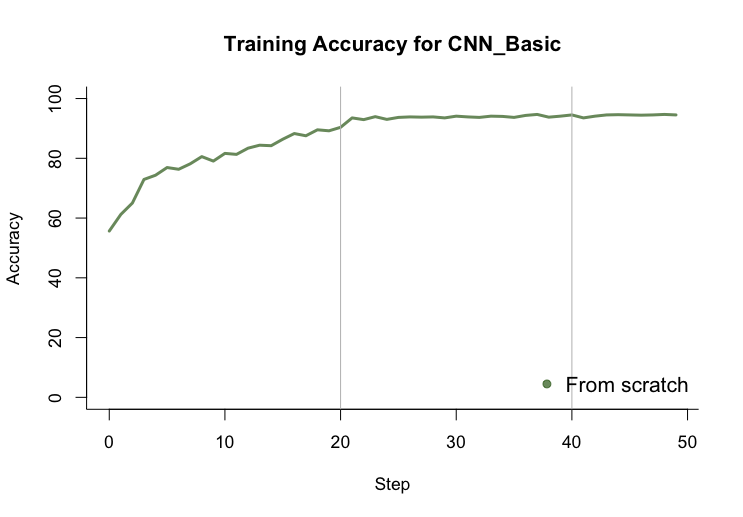
\includegraphics[width=.46\textwidth]{images/chapter5/TrainAccuracy.png}
}
\subfigure{
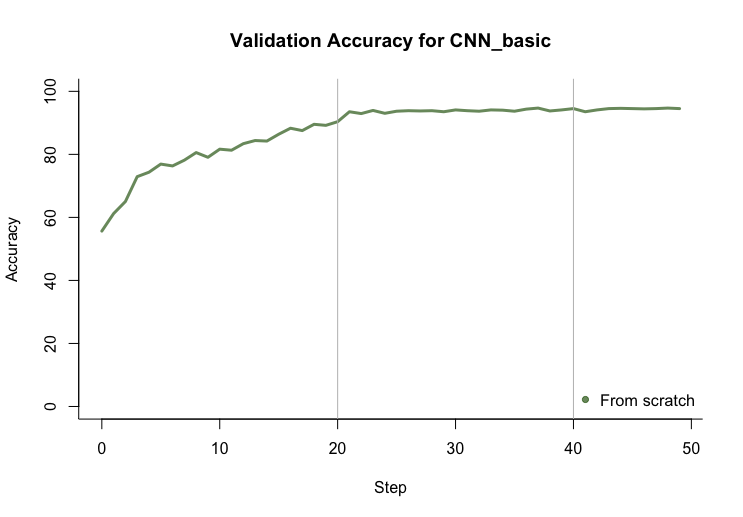
\includegraphics[width=.46\textwidth]{images/chapter5/ValAccuracy.png}
}
\caption{Training and Validation accuarcies for CNN\_basic. The vertical gray lines show when the learning rate decay happens. Convergence is reached after the 30th epoch.}
\label{fig:cnn-basic}
\end{figure}


Of course, interpreting this model is very difficult due to it's resizing of the image so early. It could be possible that the model simply learns to label all the images as non-asbestos since the dataset is strongly unbalanced but looking at the confusion matrix in Figure \ref{fig:cnn-basic-cm} shows that the model does not cheat in this way and produces sound looking results.

\begin{figure}[h]
\centering
\subfigure{
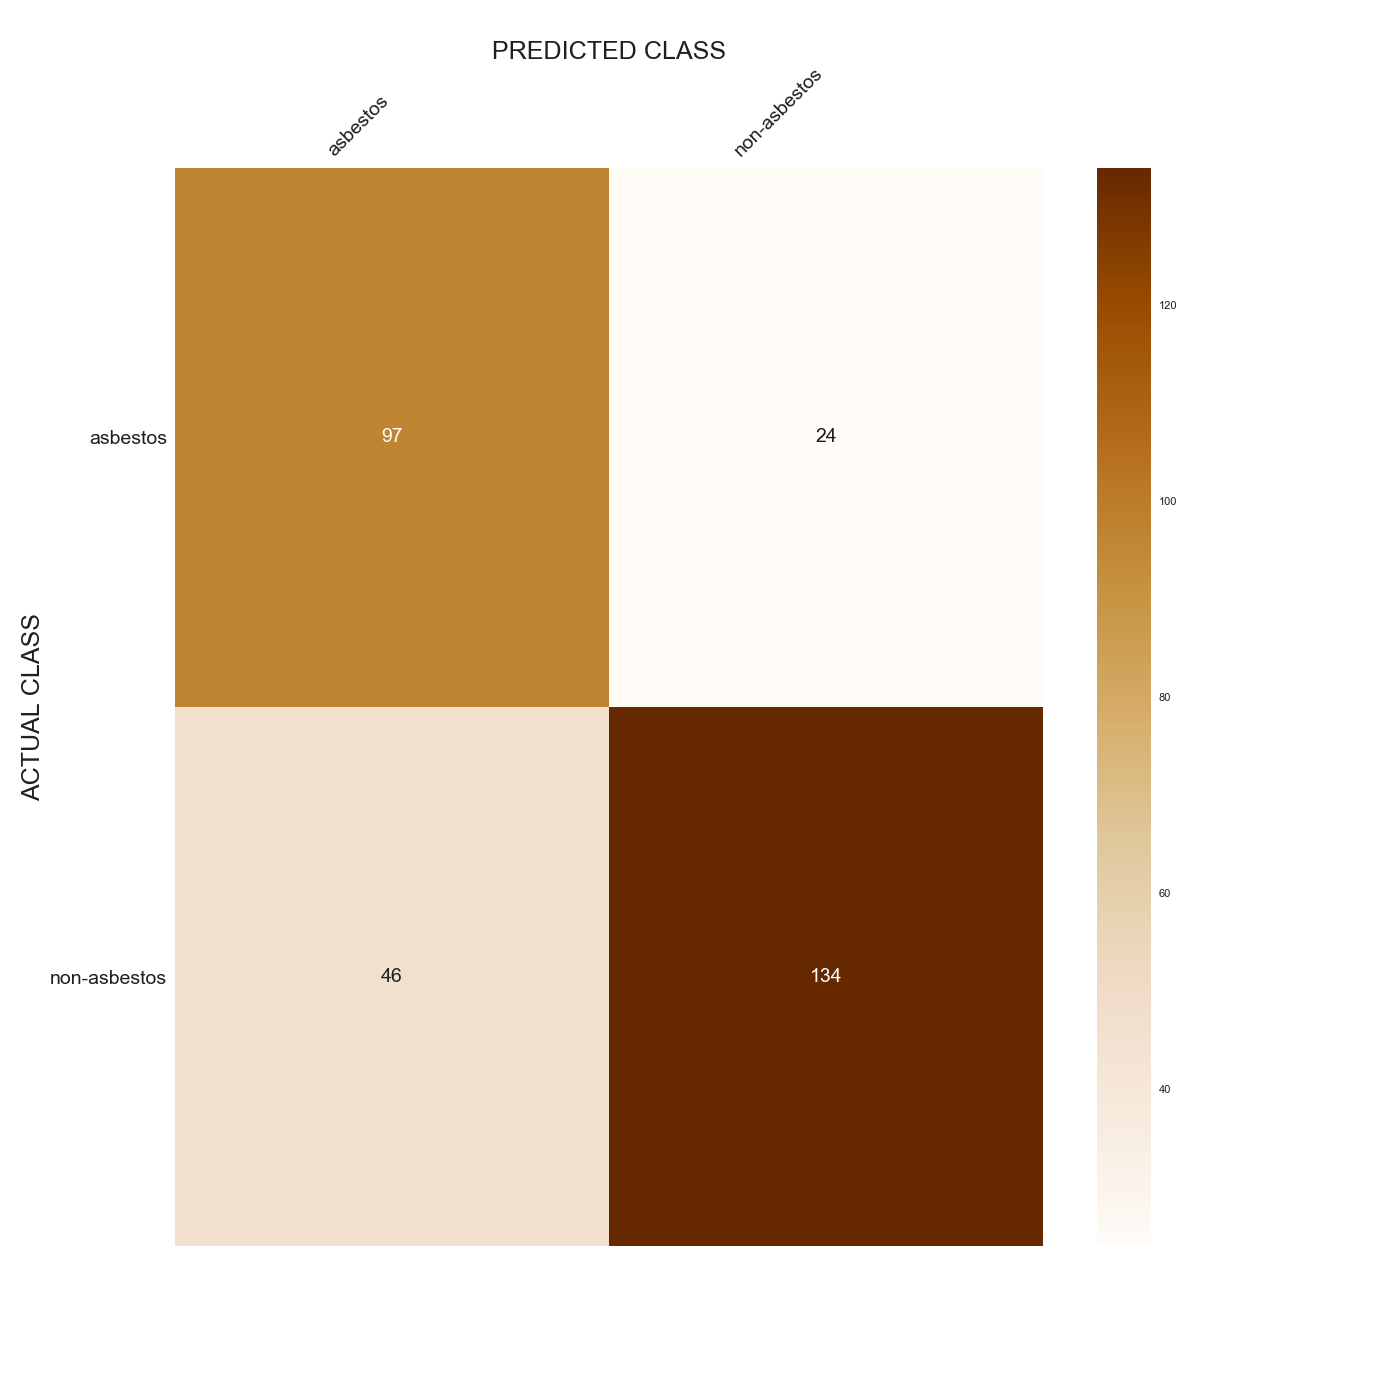
\includegraphics[width=.46\textwidth]{images/chapter5/cnn-basic-cm.png}
}
\caption{Confusion matrix of the CNN\_basic shows that the learning seems to be correct with images seperated into the two classes of asbestos and non-asbestos.}
\label{fig:cnn-basic-cm}
\end{figure}

From the confusion matrix, we can deduce type I and type II errors. Type I errors are false positives which is equivalent to a false alarm. In case of asbestos, it is better to classify wrongly some structures as asbestos than missing them which would be a type II error or a miss. Recall shows how many positive samples were actually classified as positive which in our case should be as near to 100\% as possible because it brings the type II error in relation to the overall positive samples. Recall is at 80.17\%. Precision on the other hand, how many of the predicted positive sample indeed are positive. If that number is lower, it is less severe because it simply means that more samples were classified as containing asbestos than really is the case (false alarm). Precision is at 67.83\%








%%%%%%%%%%%%%%%%%%%%%%%%%%%%%%%%%%%%%%%%%%%
%%%%%%%%%%%%%%%    ALEXNET    %%%%%%%%%%%%%%%%%%%%
%%%%%%%%%%%%%%%%%%%%%%%%%%%%%%%%%%%%%%%%%%%






\subsection{AlexNet}

AlexNet was optimized with grid search and additionally with SigOpt. With grid search the best accuracy is 81.06\% as seen in table \ref{tbl:alexnet-baseline}. It was achieved with a learning rate of 0.0001 and a learning rate decay of 20. Interestingly the SigOpt also achieved the same accuracy with a learning rate of 0.038984, a momentum of 0.073145 and a weight decay of 0.004074 as seen in table \ref{tbl:alexnet-baseline}.


\begin{table*}[h]
    \ra{1.3}
    \caption{Accuracy (\%) for several learning rates and lr-decays for AlexNet as a baseline.}
    \centering
    \begin{small}
    \textsc{
      \resizebox{0.99\textwidth}{!}{%
      \begin{tabular}{rcclcclcc}
      \toprule 
      & \multicolumn{2}{c}{Learning-Rate decay: 10} && %
        \multicolumn{2}{c}{Learning-Rate decay: 15} && %
        \multicolumn{2}{c}{Learning-Rate decay: 20} \\
      \cmidrule{2-3} \cmidrule{5-6}  \cmidrule{8-9}
      & learning rate & accuracy  && %
        learning rate & accuracy  && %
        learning rate & accuracy  \\ 
      \midrule
      AlexNet        & 0.1 & 59.80\%  &&  0.1 & 59.80\% &&  0.1 & 60.47\% \\
      AlexNet        & 0.05 & 59.80\%  &&  0.05 & 59.80\% && 0.05 & 59.80\% \\
      AlexNet        & 0.01 & 59.80\%  &&  0.01 & 59.80\% &&  0.01 & 59.80\% \\
      AlexNet        & 0.005 & 59.80\%  &&  0.005 & 59.80\% &&  0.005 & 59.80\% \\
      AlexNet        & 0.001 & 74.75\%  &&  0.001 & 77.74\% &&  0.001 & 78.74\% \\
      AlexNet        & 0.0005 & 78.74\%  &&  0.0005 & 80.40\% &&  0.0005 & 76.74\% \\
      AlexNet        & 0.0001 & 74.75\%  &&  0.0001 & 80.07\% &&  \textbf{0.0001} & \textbf{81.06\%} \\
    \bottomrule
    \end{tabular}}
    }
    \end{small}
    %\end{center}
    \vspace{-3.9mm}
    \label{tbl:alexnet-baseline}
\end{table*}

\subsection{Transfer learning on AlexNet}

When using weights from pre-training on ImageNet, the overall accuracy does get slightly better, although the increase of 0.6645\% could be due to chance. In order to show if pre-training really helps with AlexNet, each model has been run 5 times and the results are averaged as seen in Table \ref. A t-test has been run to show it's significance [NEEDS TO BE DONE]

\begin{table}[h] \centering
\ra{1.3}
\caption{Hyper parameters for Alexnet optimized with SigOpt and without pre-training}
\resizebox{0.99\textwidth}{!}{%
\begin{tabular}{@{}rrrrrrr@{}}
\toprule & learning rate & momentum & weight\_decay & lr-decay & accuracy & $\Delta$ \\
\midrule
AlexNet     from scratch    & 0.038498 & 0.073146 &  0.004074 & 20 & 81.0631\%  &         \\
AlexNet     pre-trained    & 0.034288 & 0.409378 &  0.005959 & 20 & 81.7276\%  & + 0.6645\\
\bottomrule
\end{tabular}}
\label{tbl:AlexNetBaseline}
\end{table}

\begin{table}[h] \centering
\ra{1.3}
\caption{Hyper parameters for Alexnet optimized with SigOpt and without pre-training}
\resizebox{0.99\textwidth}{!}{%
\begin{tabular}{@{}rrrrrrr@{}}
\toprule & learning rate & momentum & weight\_decay & lr-decay & accuracy & $\Delta$ \\
\midrule
AlexNet     from scratch    & 0.038498 & 0.073146 &  0.004074 & 20 & 78.61$\pm$1.16  & -     \\
AlexNet     pre-trained    & 0.034288 & 0.409378 &  0.005959 & 20 & 79.67$\pm$1.08  & - \\
AlexNet from scratch (Adam Optimizer) & 0.038498 & Adam & Adam & 20 & 59.80$\pm$0.0 & \\
\bottomrule
\end{tabular}}
\label{tbl:AlexNetMultiRun}
\end{table}

In Figure \ref{fig:alexnet-graph} we see the training and validations accuracies plotted over epochs. It can be observed that convergence is not faster with pre-training than without pre-training. Both final accuracies are almost identical. The gray vertical lines separate the graph into segments with different learning rates. So the learning rate decay happens a first time at epoch 20 and a second time at epoch 40. Convergence can be easily observed when the validation accuracy does not change anymore. Another important thing to notice is that validation and training accuracies are quite near to each other. This means that during training no severe overfitting occurred and that the validation set and train set are indeed very representative of each other. Since the final accuracy is also very near to these values it is save to say that validation and test sets are good representations of the test set and that generalizability has low variance [IF GENERALIZABILITY CAN HAVE A VARIANCE AT ALL... TODO: READ IT UP].

\begin{figure}[h]
\centering
\subfigure{
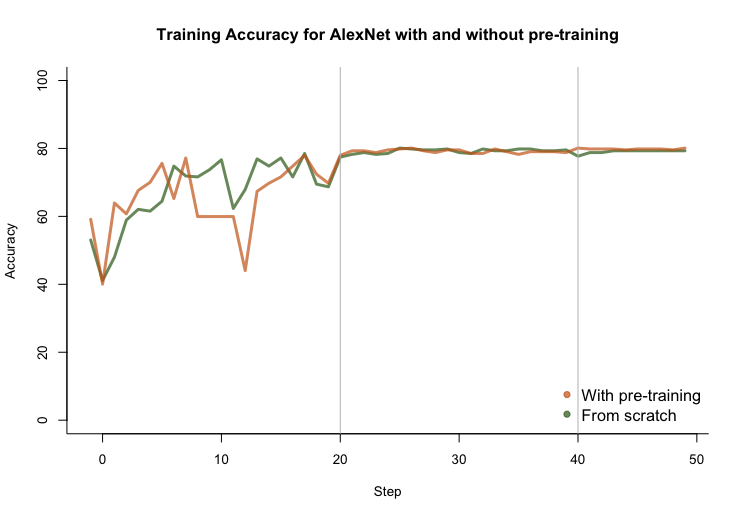
\includegraphics[width=.46\textwidth]{images/chapter5/TL/AlexNet/TA-AlexNet.png}
}
\subfigure{
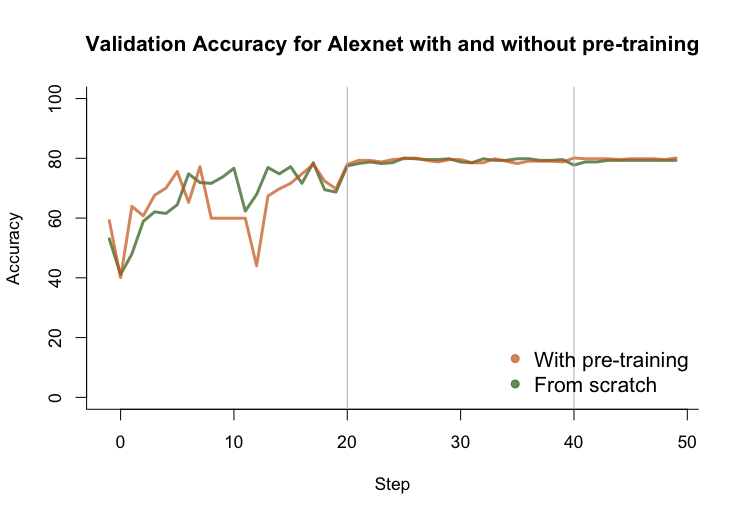
\includegraphics[width=.46\textwidth]{images/chapter5/TL/AlexNet/VA-AlexNet.png}
}
\caption{No clear difference can be observed between the pre-trained AlexNet and the not pre-trained AlexNet. Both converge roughly equally and reach almost the same final accuracy.}
\label{fig:alexnet-graph}
\end{figure}

In Figure \ref{fig:alexnet-cm} the confusion matrix of the final test set is shown for both models (pre-trainend and non pre-trained). 

\begin{figure}[h]
\centering
\subfigure{
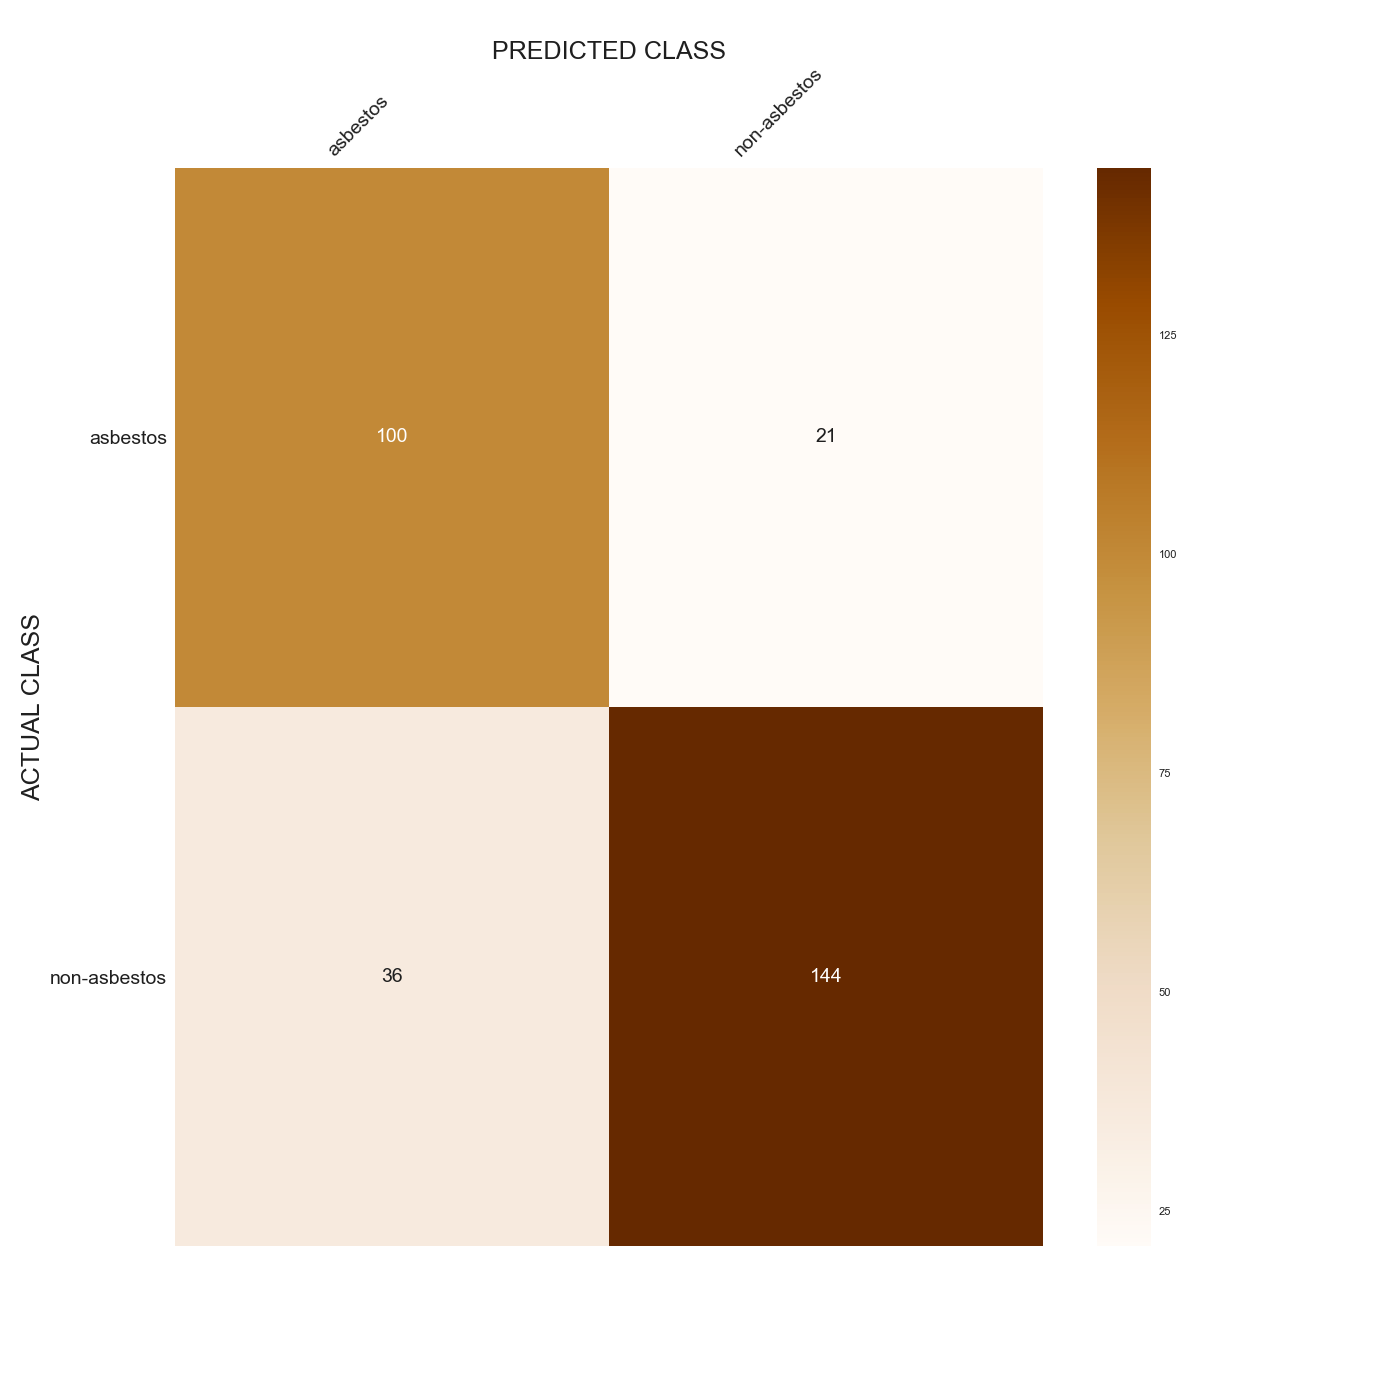
\includegraphics[width=.46\textwidth]{images/chapter5/TL/AlexNet/cm-alexnet.png}
}
\subfigure{
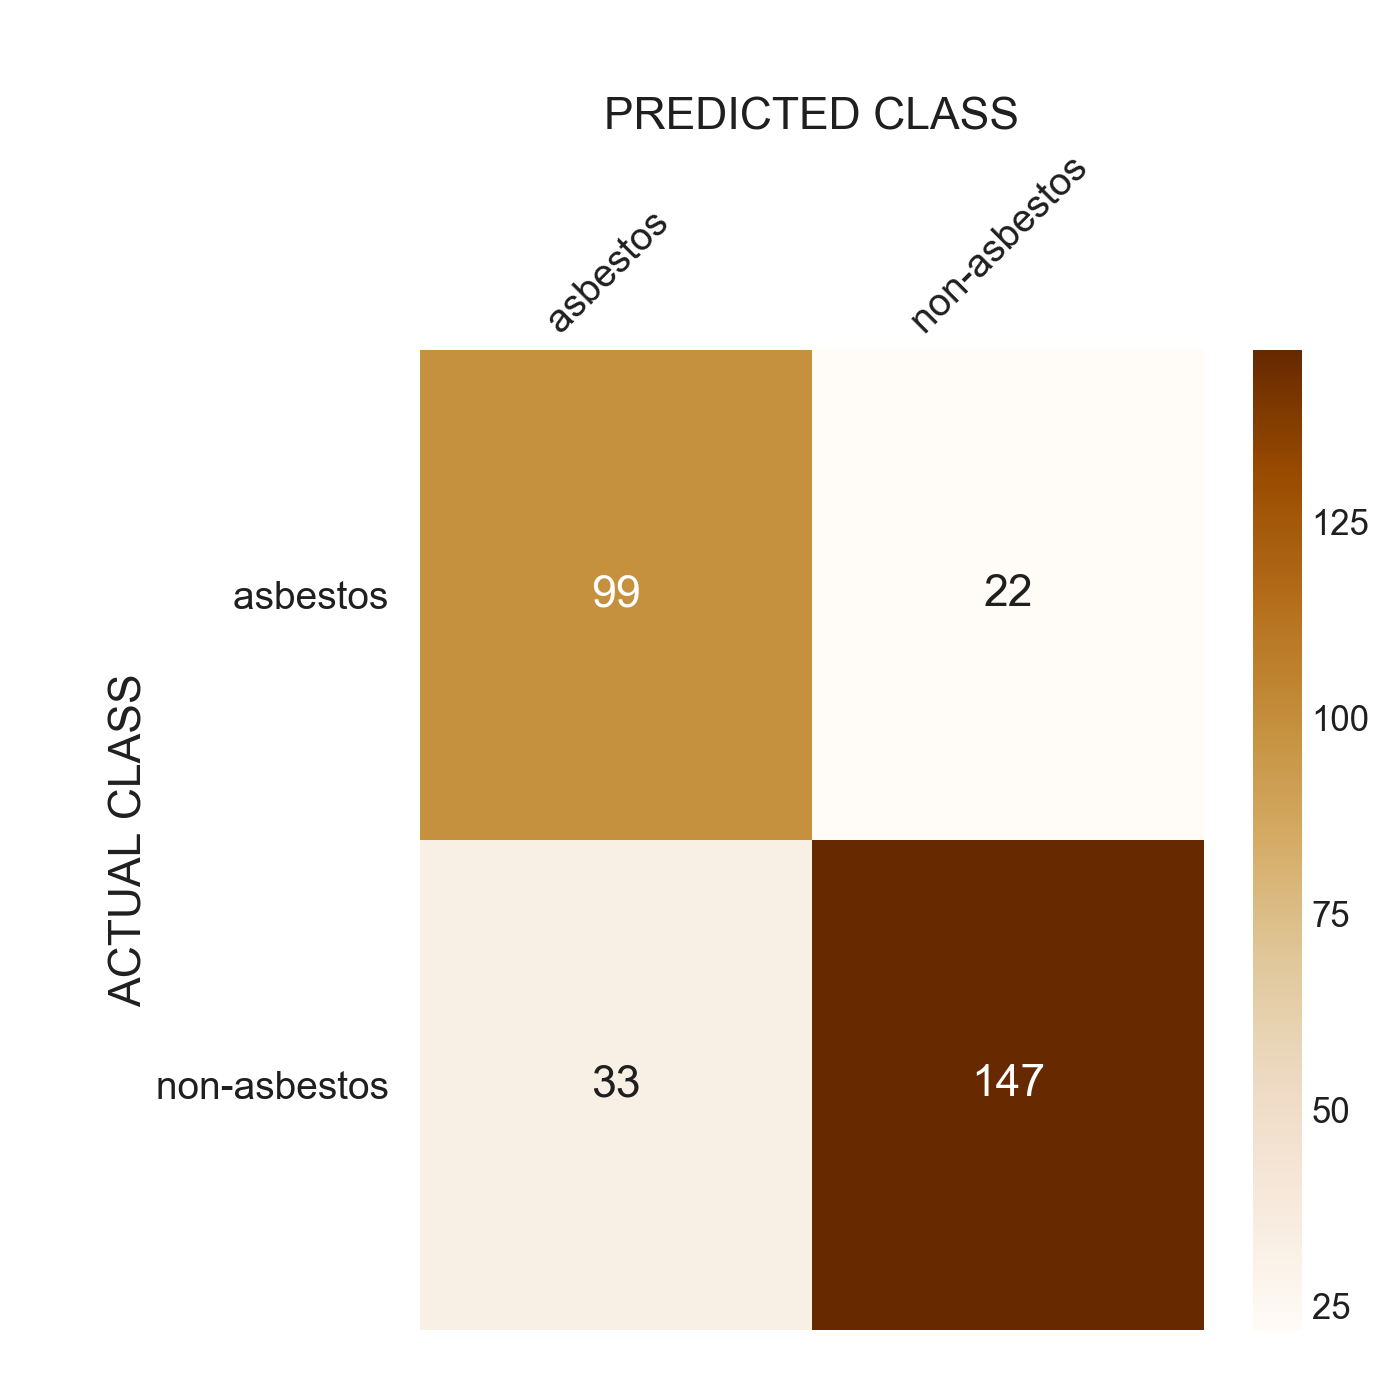
\includegraphics[width=.46\textwidth]{images/chapter5/TL/AlexNet/cm-alexnet-pre.png}
}
\caption{Confusion matrix from the model trained from scratch on the left side, and the model with pre-trained weights on the right.}
\label{fig:alexnet-cm}
\end{figure}








%%%%%%%%%%%%%%%%%%%%%%%%%%%%%%%%%%%%%%%%%%%
%%%%%%%%%%%%%%%%    VGG    %%%%%%%%%%%%%%%%%%%%%
%%%%%%%%%%%%%%%%%%%%%%%%%%%%%%%%%%%%%%%%%%%








\section{VGG}

For the following VGG architectures, the hyperparameter optimization was done with SigOpt. Every architecture was performed with and without batch normalization as well as with and without pre-training. Table XXX summarizes the results from architectures with the common depths of 11, 13, 16 and 19.

\begin{table}[h] \centering
\ra{1.3}
\caption{Hyper parameters for VGG11 and VGG11 with Batch Normalization (bn) optimized with SigOpt. First row shows hyperparameters training the architecture from scratch. Second row used pre-trained weights from ImageNet}
\resizebox{0.99\textwidth}{!}{%
\begin{tabular}{@{}rrrrrrr@{}}
\toprule & learning rate & momentum & weight\_decay & lr-decay & accuracy & $\Delta$ \\
\midrule
VGG11     from scratch    & 0.026981 & 0.743190 &  0.01 & 20 & 80.7309\%  &         \\
VGG11     pre-trained    &     0.006787 & 0.696714 &      0.01 & 20 & 88.0399\%  & +7.309 \\
\midrule
VGG11\_bn     from scratch    &     0.059343 & 0.120718 &  0.009362 & 20 & 81.0631\%  &         \\
\textbf{VGG11\_bn     pre-trained}    &     \textbf{0.022571} & \textbf{0.383537} &  \textbf{0.001733} & \textbf{20} &  \textbf{89.7010\%} & \textbf{+8.6379} \\
\bottomrule
\end{tabular}}
\label{tbl:VGG11}
\end{table}

Next, we look at VGG13 with and without batch normalization and with and without transfer-learning.

\begin{table}[h] \centering
\ra{1.3}
\caption{Hyper parameters for VGG13 and VGG13 with Batch Normalization (bn) optimized with SigOpt. First row shows hyperparameters training the architecture from scratch. Second row used pre-trained weights from ImageNet}
\resizebox{0.99\textwidth}{!}{%
\begin{tabular}{@{}rrrrrrr@{}}
\toprule & learning rate & momentum & weight\_decay & lr-decay & accuracy & $\Delta$ \\
\midrule
VGG13     from scratch    & 0.033844 & 0.257538 &  0.01 & 20 & 81.0631\%  &         \\
VGG13     pre-trained    &     0.020012 & 0.193932 & 0.01 & 20 & 88.7043\%  & +7.6412 \\
\midrule
VGG13\_bn     from scratch    &     0.054173 & 0.643504 &  0.003223 & 20 & 81.7276\%  &         \\
\textbf{VGG13\_bn     pre-trained}    &     \textbf{0.093533} & \textbf{0.041074} &  \textbf{0.009734} & \textbf{20} & \textbf{90.3655\%}  & \textbf{+8.6379} \\
\bottomrule
\end{tabular}}
\label{tbl:VGG13}
\end{table}

Next, we look at VGG16 with and without batch normalization and with and without transfer-learning.

\begin{table}[h] \centering
\ra{1.3}
\caption{Hyper parameters for VGG16 and VGG16 with Batch Normalization (bn) optimized with SigOpt. First row shows hyperparameters training the architecture from scratch. Second row used pre-trained weights from ImageNet}
\resizebox{0.99\textwidth}{!}{%
\begin{tabular}{@{}rrrrrrr@{}}
\toprule & learning rate & momentum & weight\_decay & lr-decay & accuracy & $\Delta$ \\
\midrule
VGG16     from scratch    & 0.019590 & 0.383297 &  0.00001 & 20 & 81.7276\%  &         \\
VGG16     pre-trained    &     - & - & 0.01 & 20 & -\%  & + \\
\midrule
VGG16\_bn     from scratch    &     - & - &  - & 20 & -\%  &         \\
VGG16\_bn     pre-trained    &     0.083995 & 0.242109 &  0.002634 & 20 & 89.0366\%  & + \\
\bottomrule
\end{tabular}}
\label{tbl:VGG16}
\end{table}




%%%%%%%%%%%%%%%%%%%%%%%%%%%%%%%%%%%%%%%%%%%
%%%%%%%%%%%%%%%    RESNET18    %%%%%%%%%%%%%%%%%%%
%%%%%%%%%%%%%%%%%%%%%%%%%%%%%%%%%%%%%%%%%%%








\section{ResNet18}

For ResNet18 only SigOpt was used for tuning the hyperparameters. It was used for training the architecture from scratch and with pre-trained weights. Table \ref{tbl:ResNet18} shows a summary of the optimization process with the best accuracies and the delta between the pre-trained model and the model trained from scratch.

\begin{table}[h] \centering
\ra{1.3}
\caption{Hyper parameters for ResNet18 optimized with SigOpt. First row shows hyperparameters training the architecture from scratch. Second row used pre-trained weights from ImageNet}
\resizebox{0.99\textwidth}{!}{%
\begin{tabular}{@{}rrrrrrr@{}}
\toprule & learning rate & momentum & weight\_decay & lr-decay & accuracy & $\Delta$ \\
\midrule
ResNet18     from scratch    & 0.033678 & 0.952630 &  0.007518 & 20 & 83.0565\%  &         \\
ResNet18     pre-trained    &     0.039918 & 0.170826 &  0.001980 & 20 & 88.0399\%  & + 4.9834\\
\bottomrule
\end{tabular}}
\label{tbl:ResNet18}
\end{table}

The graphs in Figure \ref{fig:resnet18-graph} show clearly that training converged much faster for the model with pre-trained weights. After only a few epochs it reached convergence while the model without pre-trained weights had to catch up over many epochs and actually overfitted to the training data somewhere after epoch 30. The validation error started to slightly decrease for the model trained from scratch while the training accuracy kept climbing. That is bad and is also reflected in the final accuracies.

\begin{figure}[h]
\centering
\subfigure{
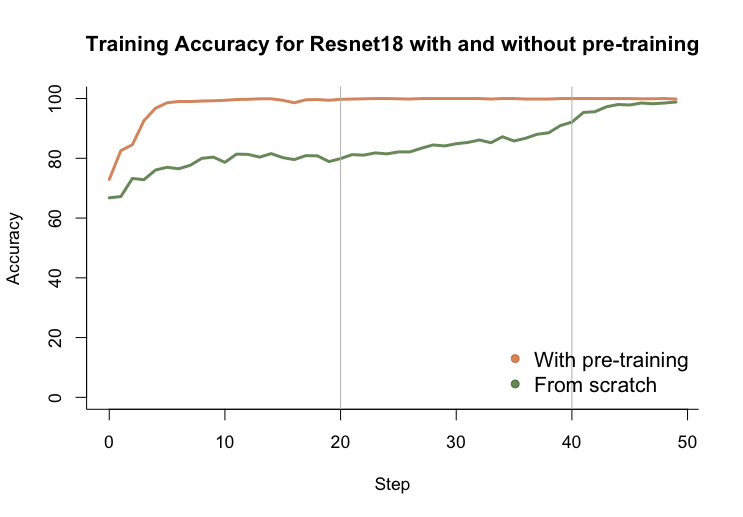
\includegraphics[width=.46\textwidth]{images/chapter5/TL/ResNet18/TA-ResNet18.png}
}
\subfigure{
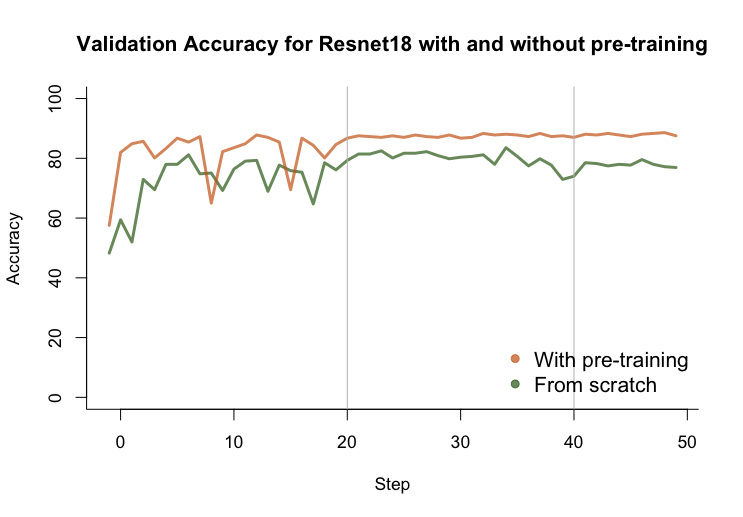
\includegraphics[width=.46\textwidth]{images/chapter5/TL/ResNet18/VA-ResNet18.png}
}
\caption{Training and validation graphs for ResNet18 once with pre-trained weights from ImageNet and once trained from scratch.}
\label{fig:resnet18-graph}
\end{figure}

With the confusion matrix in Figure \ref{resnet18-cm} we can see that the learning did not take any shortcuts and that the distinction between images with asbestos fibers and images without were clearly separated to some extent that is reflected in the overall accuracy reached. The Precision and Recall for the model trained from scratch are 77.78\% and 80.99\%, respectively. For model with pre-trained weight, Precision and Recall are much better with 83.47\% and 87.60\%, respectively.

\begin{figure}[h]
\centering
\subfigure{
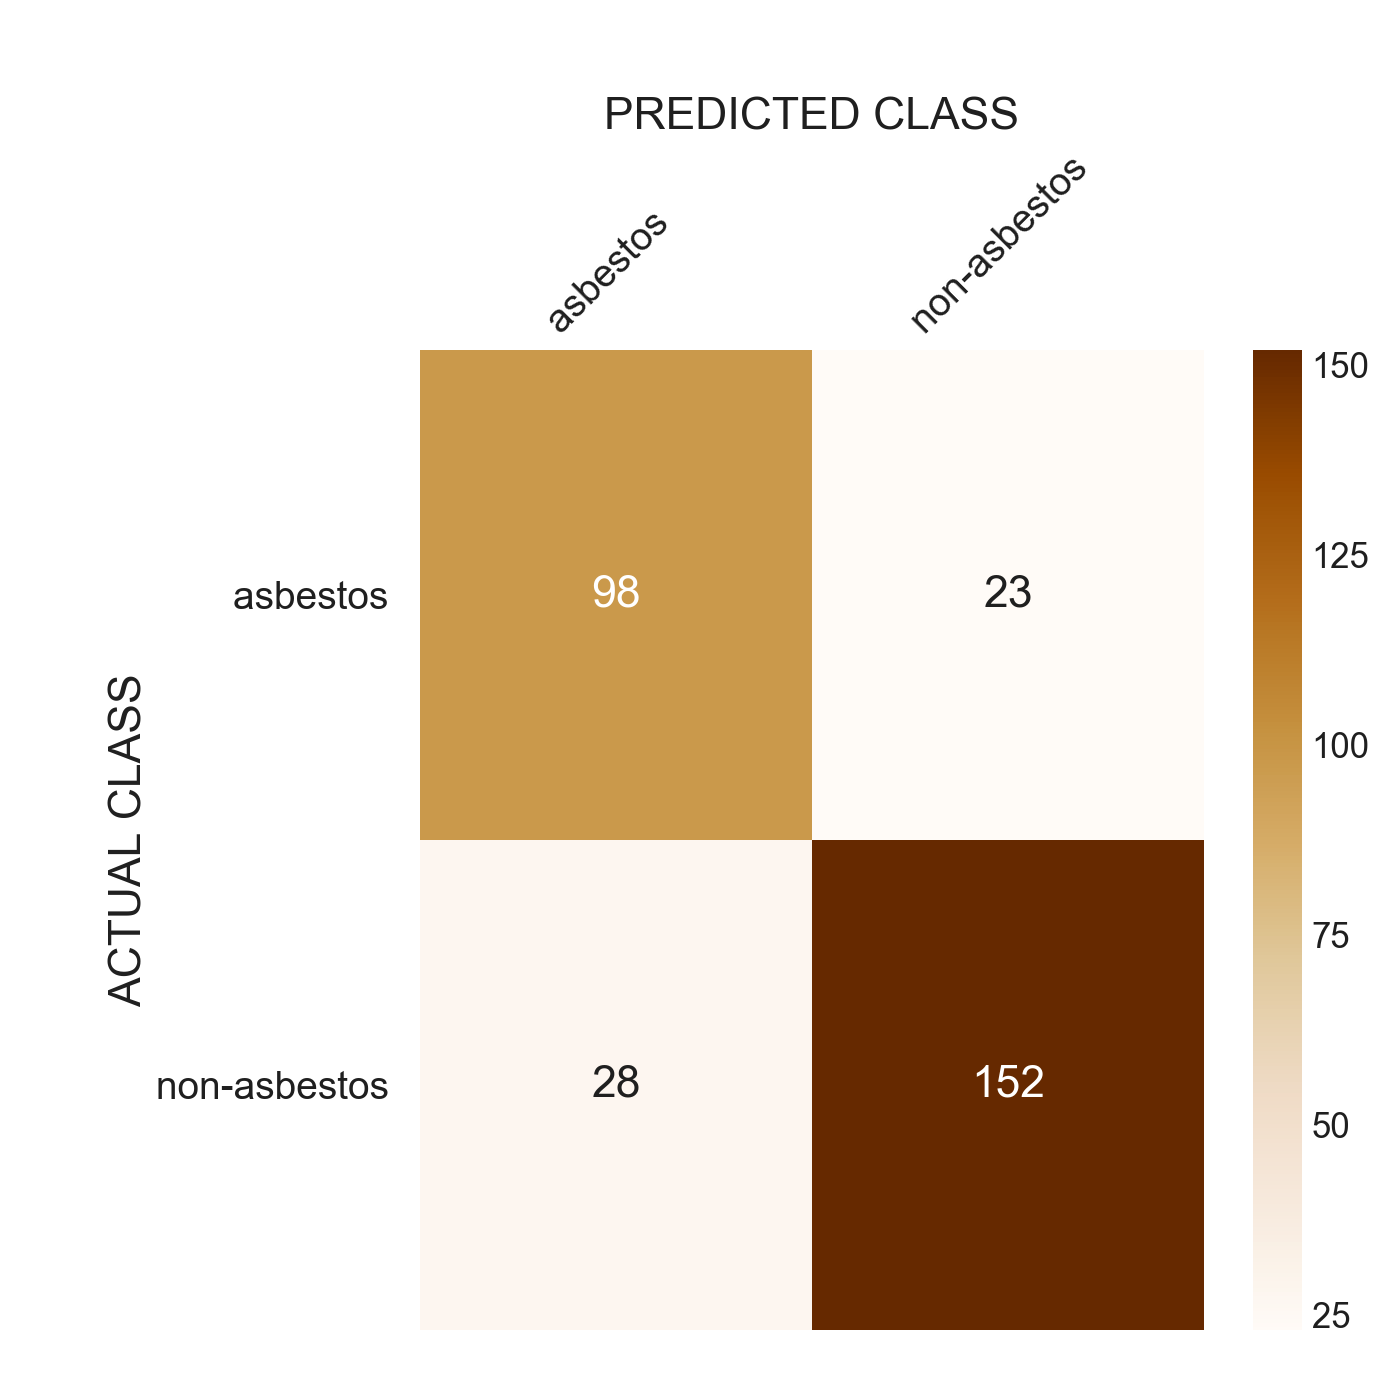
\includegraphics[width=.46\textwidth]{images/chapter5/TL/ResNet18/cm-resnet18.png}
}
\subfigure{
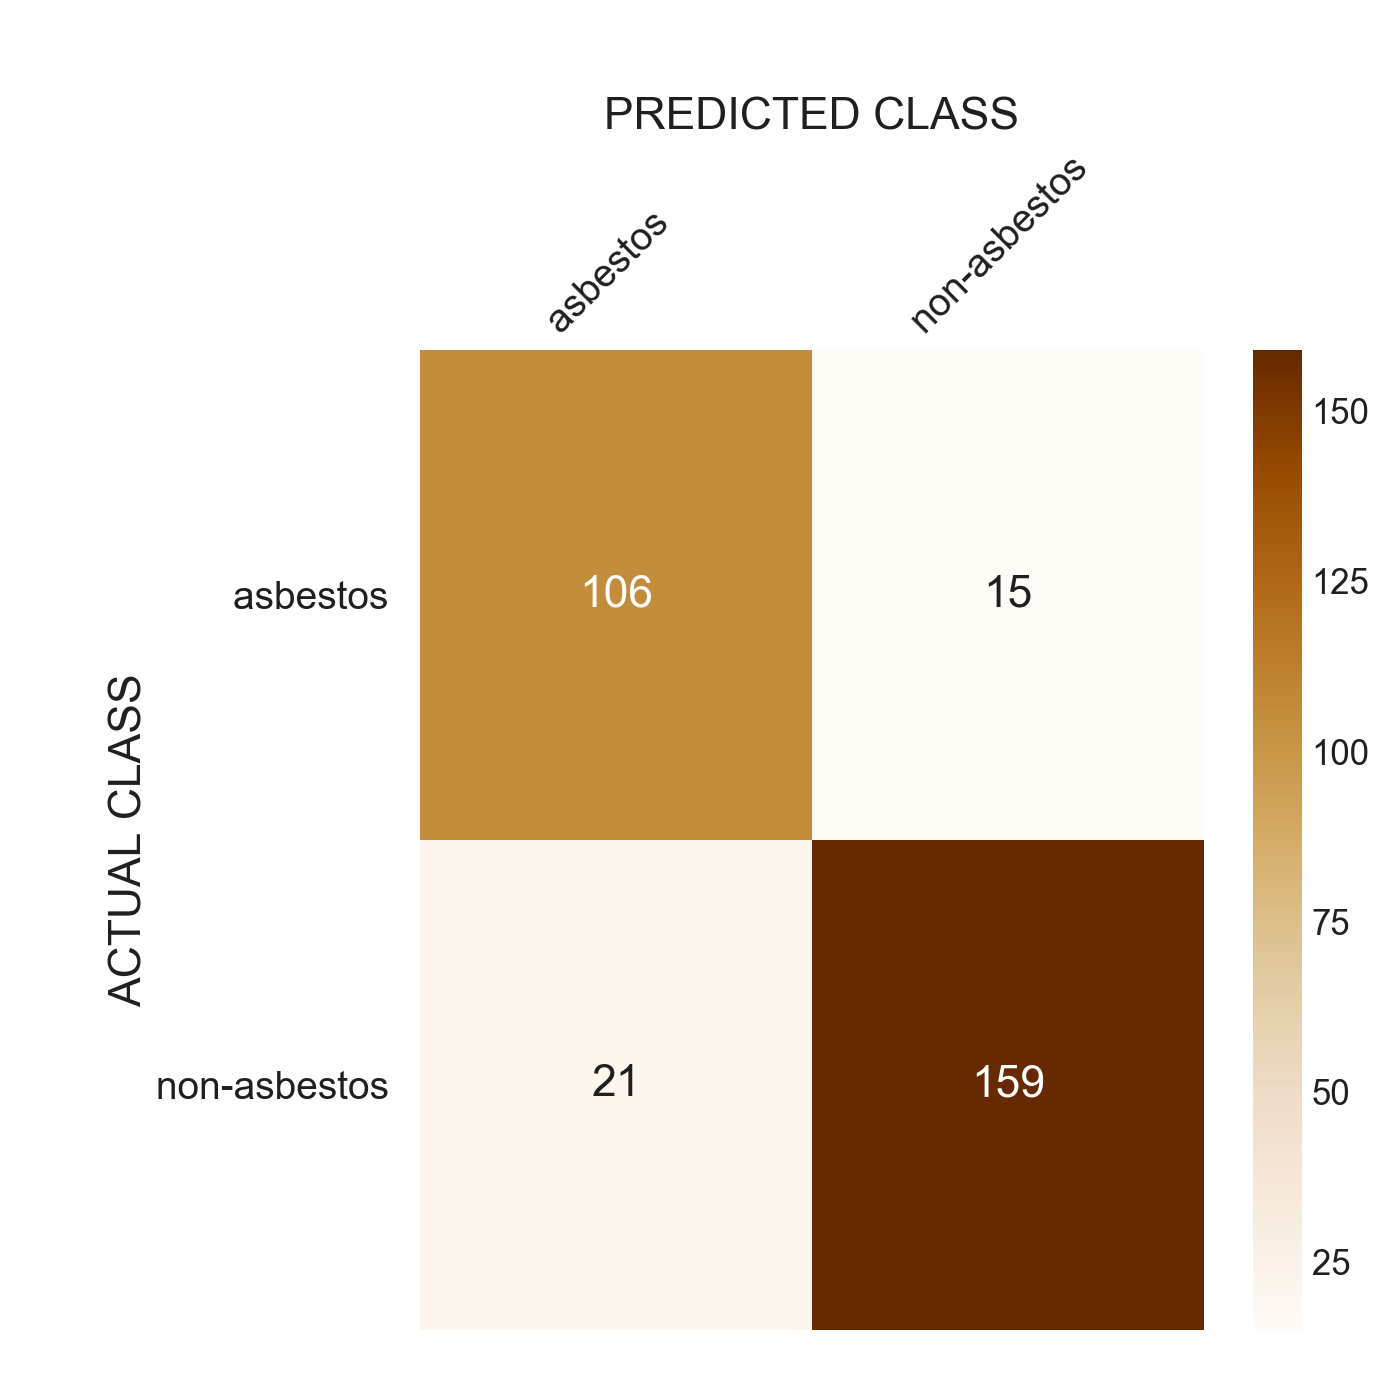
\includegraphics[width=.46\textwidth]{images/chapter5/TL/ResNet18/cm-resnet18-pre.png}
}
\caption{On the left: confusion matrix from model trained from scratch. On the right trained with transfer learning applied.}
\label{fig:resnet18-cm}
\end{figure}







%%%%%%%%%%%%%%%%%%%%%%%%%%%%%%%%%%%%%%%%%%%
%%%%%%%%%%%%%%%    RESNET34    %%%%%%%%%%%%%%%%%%%
%%%%%%%%%%%%%%%%%%%%%%%%%%%%%%%%%%%%%%%%%%%









\section{ResNet34}

ResNet34 is a variation of the ResNet architecture and has simply more layers than the Resnet18. Hyperparameter optimization was done with SigOpt and for both variants, training from scratch and training with pre-trained weights from ImageNet.

\begin{table}[h] \centering
\ra{1.3}
\caption{Hyper parameters for ResNet34 optimized with SigOpt. First row shows hyperparameters training the architecture from scratch. Second row used pre-trained weights from ImageNet}
\resizebox{0.99\textwidth}{!}{%
\begin{tabular}{@{}rrrrrrr@{}}
\toprule & learning rate & momentum & weight\_decay & lr-decay & accuracy & $\Delta$ \\
\midrule
ResNet34     from scratch    & 0.040323 & 0.141704 &  0.004044 & 20 & 83.0565\%  &         \\
ResNet34     pre-trained    &     0.060848 & 0.460187 &  0.000537 & 20 & 87.0431\%  & +3.9866\\
\bottomrule
\end{tabular}}
\label{tbl:ResNet34}
\end{table}








%%%%%%%%%%%%%%%%%%%%%%%%%%%%%%%%%%%%%%%%%%%
%%%%%%%%%%%%%%%    DENSENET121    %%%%%%%%%%%%%%%%%
%%%%%%%%%%%%%%%%%%%%%%%%%%%%%%%%%%%%%%%%%%%









\section{Densenet121}

Hyperparameter optimization for densenet121 was done with SigOpt and for both variants, training from scratch and training with pre-trained weights from ImageNet.

\begin{table}[h] \centering
\ra{1.3}
\caption{Hyper parameters for densenet121 optimized with SigOpt. First row shows hyperparameters training the architecture from scratch. Second row used pre-trained weights from ImageNet}
\resizebox{0.99\textwidth}{!}{%
\begin{tabular}{@{}rrrrrrr@{}}
\toprule & learning rate & momentum & weight\_decay & lr-decay & accuracy & $\Delta$ \\
\midrule
Densenet121     from scratch    & 0.035925 & 0.057618 &  0.009241 & 20 & 86.0465\%  &         \\
Densenet121     pre-trained    &     0.018489     & 0.369998 &  0.004963 & 20 & 88.3721\%  & +2.3256\\
\bottomrule
\end{tabular}}
\label{tbl:Densenet121}
\end{table}





%%%%%%%%%%%%%%%%%%%%%%%%%%%%%%%%%%%%%%%%%%%
%%%%%%%%%%%%%%%    DENSENET169    %%%%%%%%%%%%%%%%%
%%%%%%%%%%%%%%%%%%%%%%%%%%%%%%%%%%%%%%%%%%%





\section{Densenet169}

Hyperparameter optimization for densenet169 was done with SigOpt and for both variants, training from scratch and training with pre-trained weights from ImageNet.

\begin{table}[h] \centering
\ra{1.3}
\caption{Hyper parameters for densenet121 optimized with SigOpt. First row shows hyperparameters training the architecture from scratch. Second row used pre-trained weights from ImageNet}
\resizebox{0.99\textwidth}{!}{%
\begin{tabular}{@{}rrrrrrr@{}}
\toprule & learning rate & momentum & weight\_decay & lr-decay & accuracy & $\Delta$ \\
\midrule
Densenet169 from scratch    & 0.005812 & 0.777249 & 0.006999  & 20 & 85.3821\%  &         \\
Densenet169 pre-trained    & 0.006347 & 0.447591 & 0.005180 & 20 & 89.3688\%  & +3.9867\\
\bottomrule
\end{tabular}}
\label{tbl:Densenet169}
\end{table}




%%%%%%%%%%%%%%%%%%%%%%%%%%%%%%%%%%%%%%%%%%%
%%%%%%%%%%%%%%%    INCEPTIONv3   %%%%%%%%%%%%%%%%%%
%%%%%%%%%%%%%%%%%%%%%%%%%%%%%%%%%%%%%%%%%%%









\section{Inception}


Hyperparameter optimization for inception v3 was done with SigOpt and for both variants, training from scratch and training with pre-trained weights from ImageNet.

\begin{table}[h] \centering
\ra{1.3}
\caption{Hyper parameters for inception v3 optimized with SigOpt. First row shows hyperparameters training the architecture from scratch. Second row used pre-trained weights from ImageNet}
\resizebox{0.99\textwidth}{!}{%
\begin{tabular}{@{}rrrrrrr@{}}
\toprule & learning rate & momentum & weight\_decay & lr-decay & accuracy & $\Delta$ \\
\midrule
Inception v3 from scratch    & 0.070046 & 0.910505 & 0.006943 & 20 & 83.3887\%  &         \\
Inception v3 pre-trained    & 0.029269 & 0.0 & 0.006320 & 20 & 88.7043\%  & +5.3156\\
\bottomrule
\end{tabular}}
\label{tbl:Inceptionv3}
\end{table}

\section{Conclusion on Transfer Learning}



